\section{Introduction}

\begin{figure*}
    \centering
    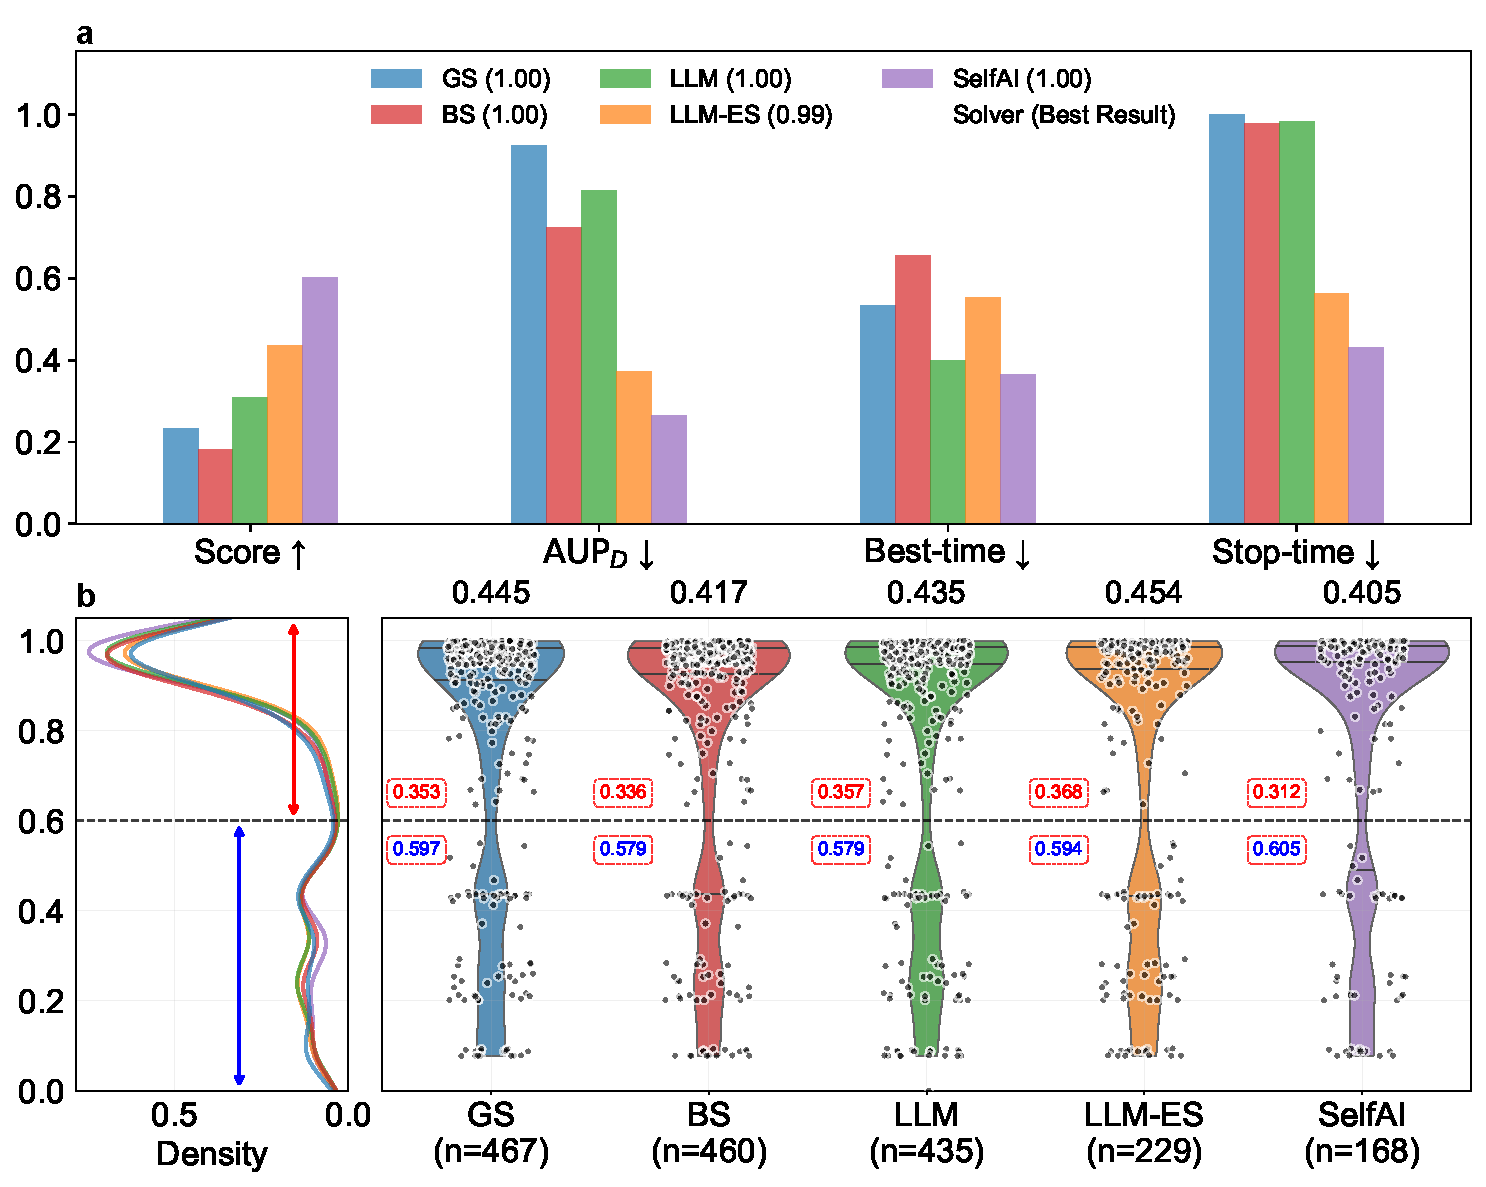
\includegraphics[width=1.0\linewidth]{figures/analysis/solver_performance_comparison2.pdf}
    \caption{\textbf{Performance comparison and efficiency-diversity trade-offs across solvers.} \textbf{a}, Normalized performance of five solvers (GS, BS, LLM, LLM-ES, and SelfAI) evaluated by Score (higher is better), $\text{AUP}_D$, Best-time, and Stop-time (lower is better). Bars indicate solver-level averages, with values in parentheses denoting the best-achieved or optimal reference performance. \textbf{b}, Outcome distributions across solvers. Left: kernel density estimates illustrating score concentration and convergence tendencies. Right: violin plots with overlaid individual trials (sample size n shown), capturing performance variability. The dashed horizontal line denotes the evaluation threshold separating low- and high-performance regimes; annotated statistics (red/blue) highlight solver behavior above and below this threshold, where broader exploration facilitates rapid escape from low-performance regions and tighter distributions in high-performance regions enable localized refinement.}
    \label{fig:comparison}
\end{figure*}

Scientific discovery across engineering~\cite{bradshaw1983studying,angelopoulos2024transforming}, physics~\cite{lupoiu2025multi,kaiser2025large}, biology~\cite{lyu2024alphafold2,nguyen2024sequence}, and medicine~\cite{yakavets2025machine,grisoni2021combining,jiang2022artificial} increasingly relies on artificial intelligence (AI) systems to support or partially automate key stages of the scientific workflow, ranging from data analysis and hypothesis generation to experimental design and execution. As scientific problems grow in scale, dimensionality, and uncertainty, computational methods have become indispensable for exploring complex hypothesis spaces. AI-assisted discovery systems hold the promise of fundamentally changing the way scientific discovery is practiced~\cite{xin2025towards}.

Most existing AI-assisted discovery systems~\cite{aira,yakavets2025machine,erps2021accelerated} adopt machine-learning-rooted paradigms, emphasizing predictive modeling on large datasets and evaluating success primarily by final performance metrics. While effective for many applications, these paradigms provide limited support for reasoning about the discovery process itself, including how hypotheses are explored, how experiments are prioritized, and how decisions are made under uncertainty. In particular, they rarely treat scientific discovery as a sequential, long-horizon decision process in which exploration strategies, resource allocation, and stopping decisions must be jointly optimized over time. Unlocking the full potential of AI in discovery, therefore, requires moving beyond performance-centric automation toward frameworks that explicitly support exploration, decision-making, and adaptation throughout the discovery trajectory.


Recent advances in large language models (LLMs)~\cite{openai2023gpt,bai2023qwen,guo2025deepseek} have significantly expanded the potential of AI systems in scientific research. Improvements in reasoning, multimodal understanding, and autonomous tool use now enable LLM-based systems to integrate planning, execution, and feedback within unified workflows. As a result, these systems can support key components of scientific discovery, including hypothesis generation, experiment design, and iterative refinement across domains~\cite{huang2022towards,ferrag2025llm}.
% 
Building on these capabilities, prior work has progressively enhanced individual aspects of the scientific workflow. Early efforts demonstrated that LLMs can extract actionable scientific knowledge to guide experiments~\cite{lin2023evolutionary,angelopoulos2024transforming} and answer domain-specific professional questions~\cite{alampara2025probing,polak2024extracting,dagdelen2024structured}. Subsequent research extended these capabilities to cross-stage planning~\cite{biomni}, automated hypothesis generation~\cite{wang2025discovery,aira,baek2025researchagent}, multimodal knowledge integration~\cite{steyaert2023multimodal,gao2025chemical}, and automated experimentation across scientific domains. These advances have led to a new generation of scientific discovery systems, ranging from AI research assistants to fully autonomous workflows capable of executing end-to-end benchmarks~\cite{king2004functional,mandal2025evaluating,ai_co_scientist}.

While these systems demonstrate the feasibility of system-level automation in scientific workflows, most existing approaches focus primarily on improving individual stages of the discovery process or optimizing final outcomes. Even recent LLM-driven optimization methods~\cite{liao2025llm4eo,jiang2025agenticsciml,kochnev2025optuna}, which infer evolutionary patterns and synthesize update rules, operate largely at the level of execution or local improvement.
% 
However, scientific discovery is inherently a sequential and strategic process that unfolds over time. It requires reasoning not only about isolated steps but also about the structure and quality of the entire exploration trajectory. Current systems rarely treat discovery as a trajectory-level decision-making problem. Consequently, they do not explicitly address fundamental challenges such as determining optimal stopping points, designing efficient exploration paths, or evaluating the structural effectiveness of discovery strategies over time.

Addressing these limitations requires a shift from execution-oriented autonomy toward cognitively oriented autonomy, in which discovery systems reason about exploration strategies, evaluate efficiency-diversity trade-offs, and adaptively decide when to stop. Motivated by this perspective, we introduce SelfAI, a self-directed, multi-agent-enabled discovery system that treats scientific discovery as a trajectory-level decision-making process. We integrate human intent, exploration reasoning, and experimental execution into a unified closed-loop framework. These are built with three modules and external tools (Fig.~\ref{fig:flowchart}a), enabling efficiency-diversity exploration in long-horizon scientific workflows. To evaluate discovery quality, we introduce two novel complementary metrics, Score (Discovery Efficiency) and $\text{AUP}_D$ (Area Under the Performance Diversity). Score aggregates across tasks, the normalized improvement over the search space together with penalties for discovering good configurations late and for stopping far from the best-found point. $\text{AUP}_D$ explicitly encodes how broadly a solver explores the search space by summarizing the performance-diversity tradeoffs across the entire trajectory, enabling detailed analysis of exploration behavior and stopping decisions in long-term searches. Together, these metrics measure quantitative assessments of exploration behavior, reasoning structure, and stopping decisions in long-term autonomous experiments.


\begin{figure*}[hbtp]
    \centering
    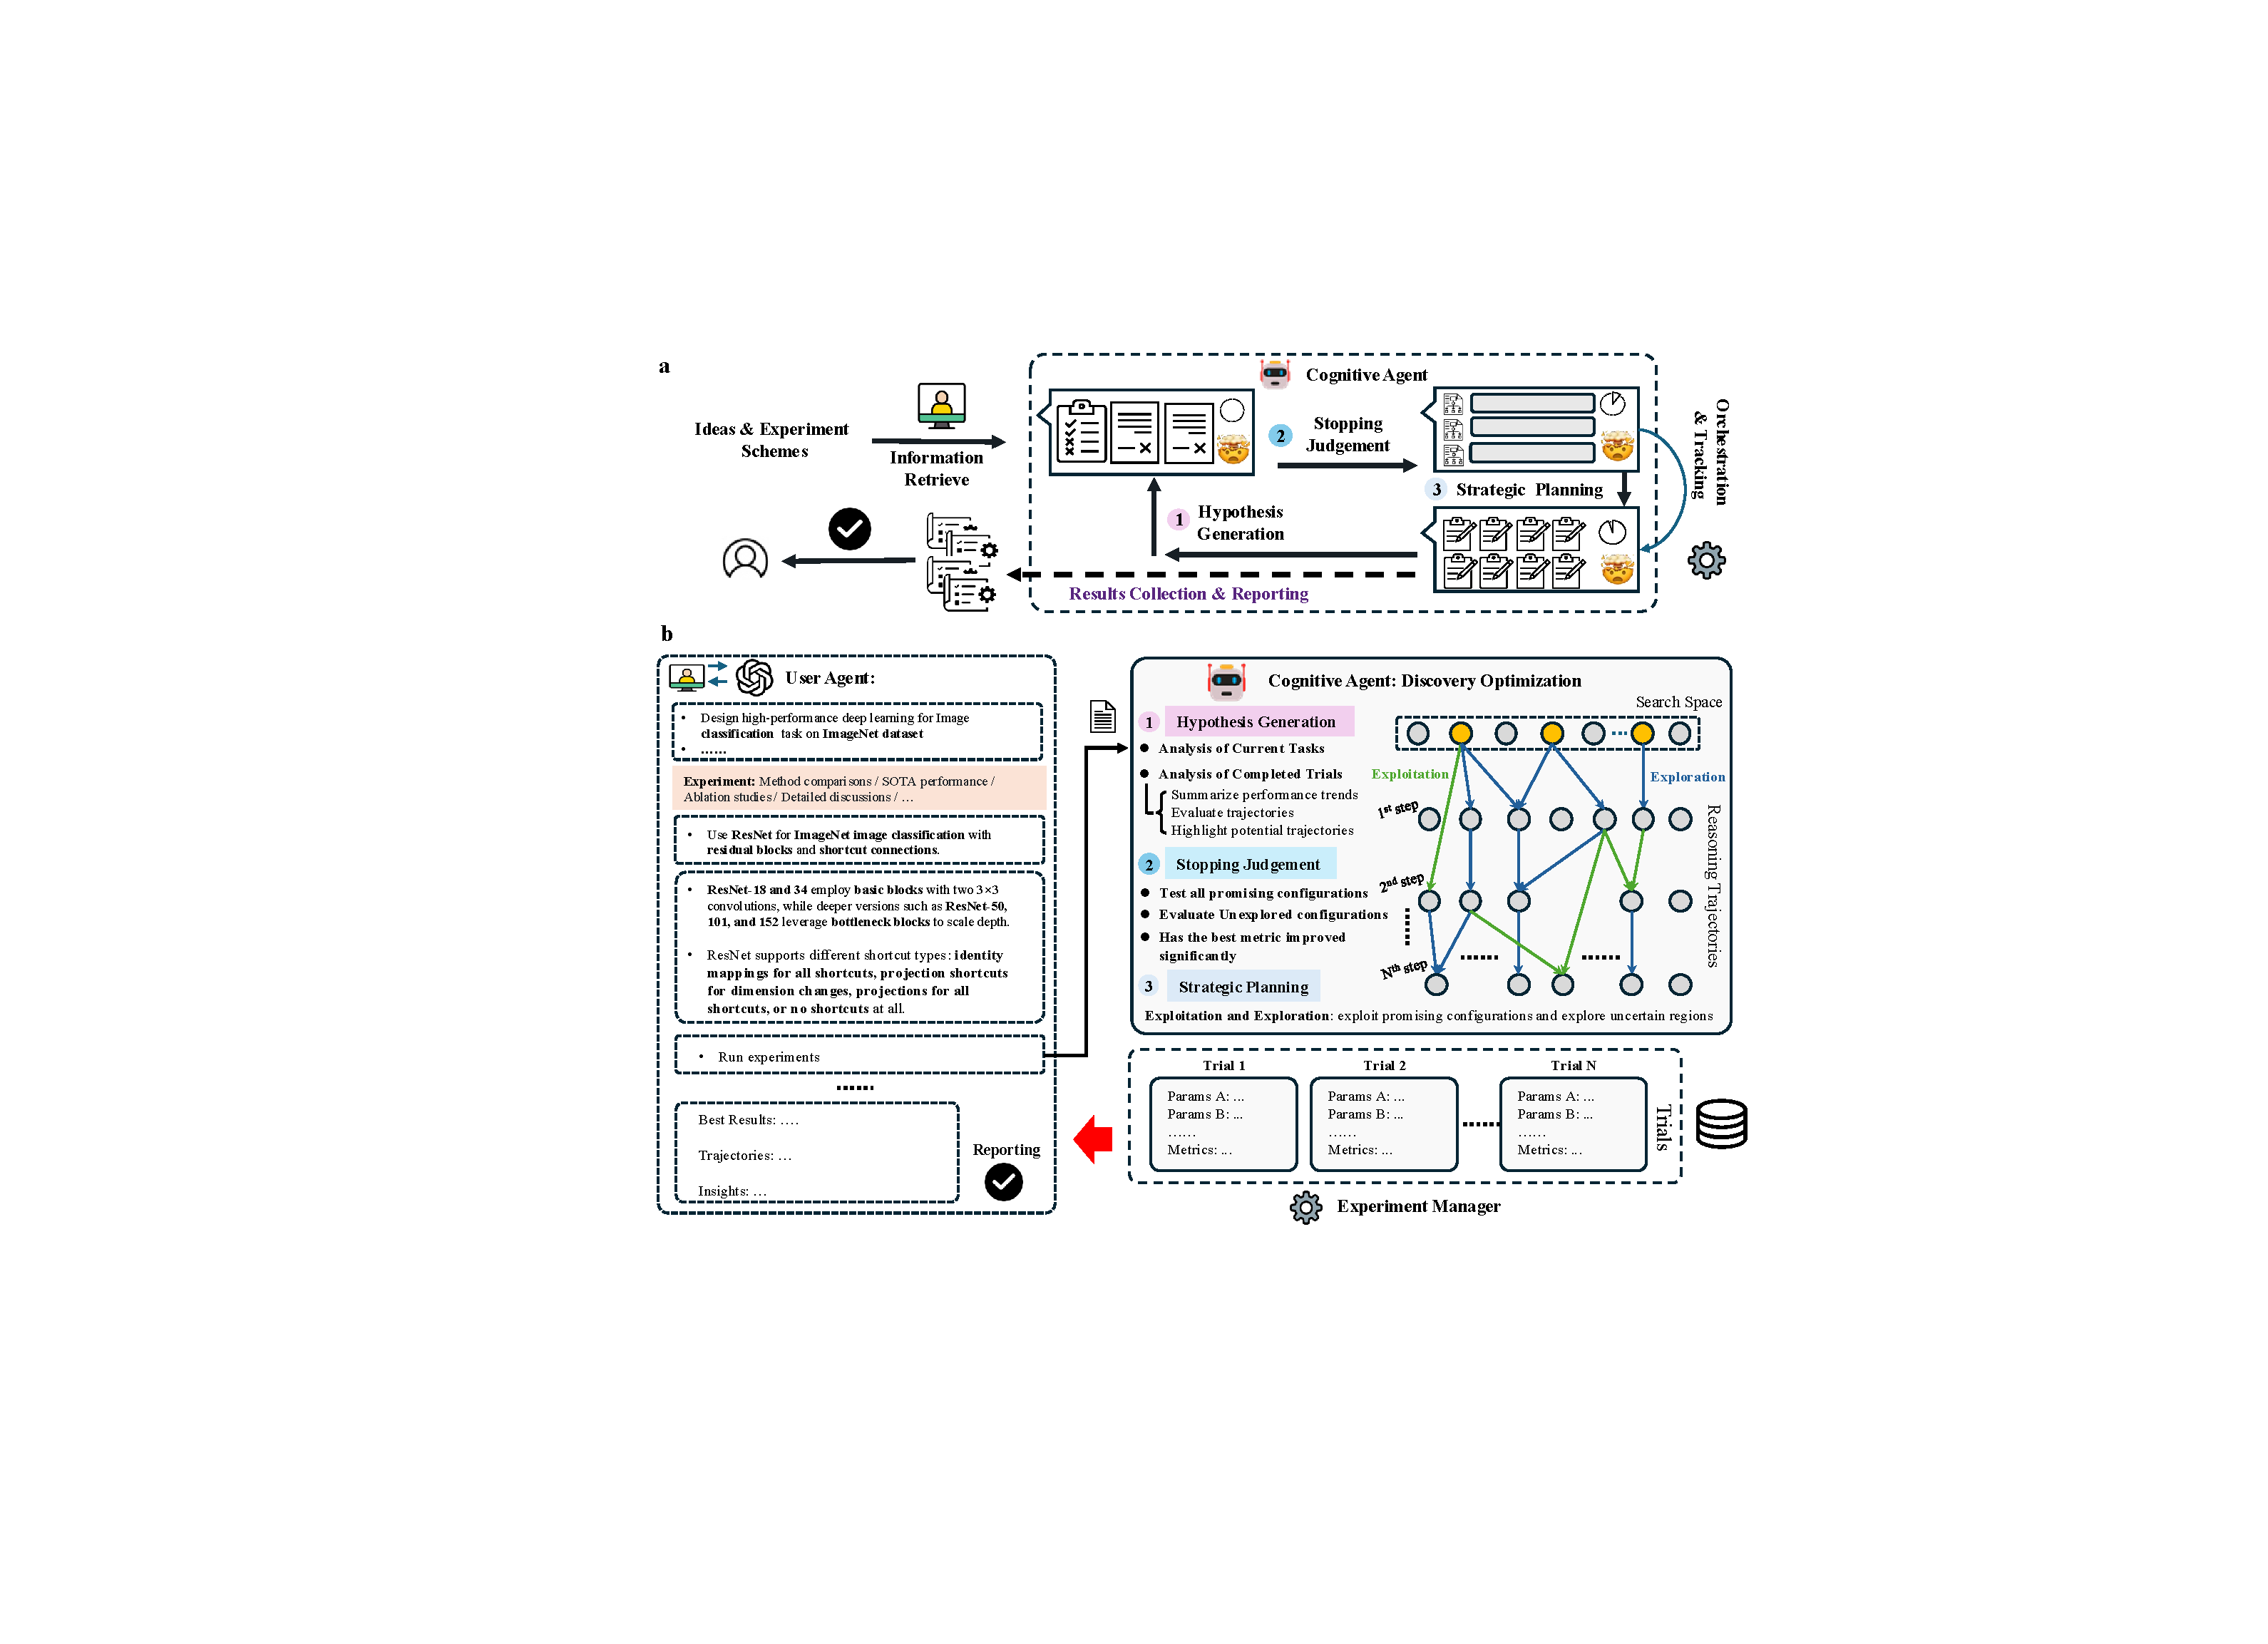
\includegraphics[width=1.0\textwidth]{figures/flowchart3-v2.pdf}
    % 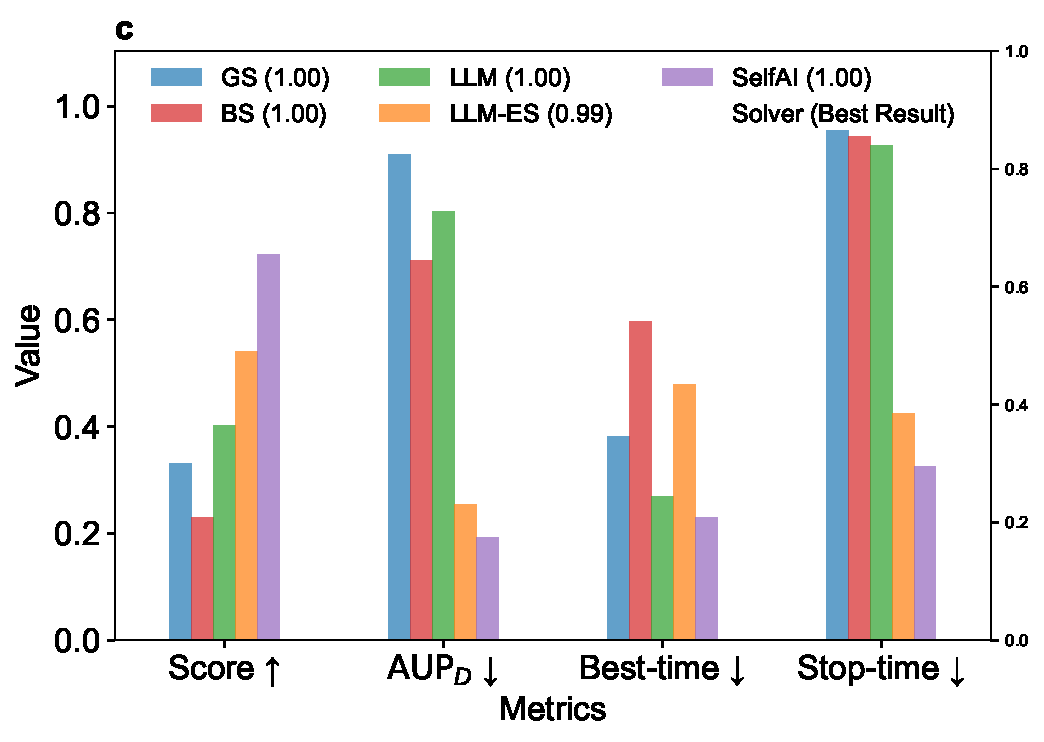
\includegraphics[width=0.49\linewidth]{figures/analysis/llm_comparison.pdf}
    % \includegraphics[width=0.49\linewidth]{figures/analysis/solver_performance_comparison.pdf}
    
    % 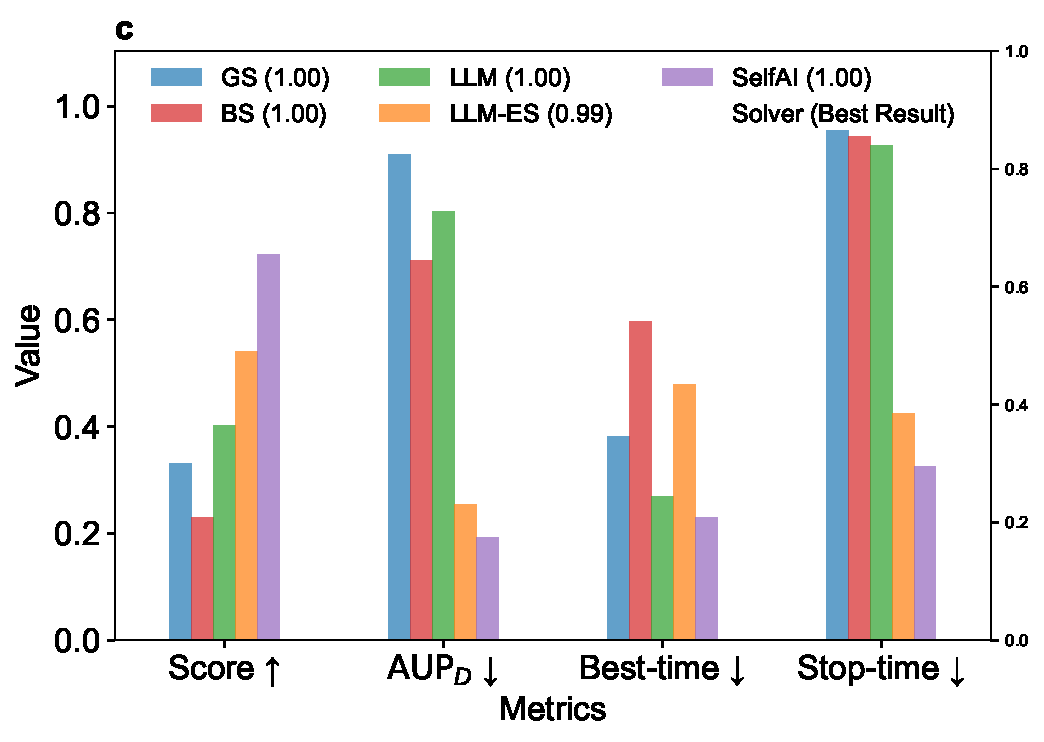
\includegraphics[width=0.7\linewidth]{figures/analysis/llm_comparison.pdf}
    % 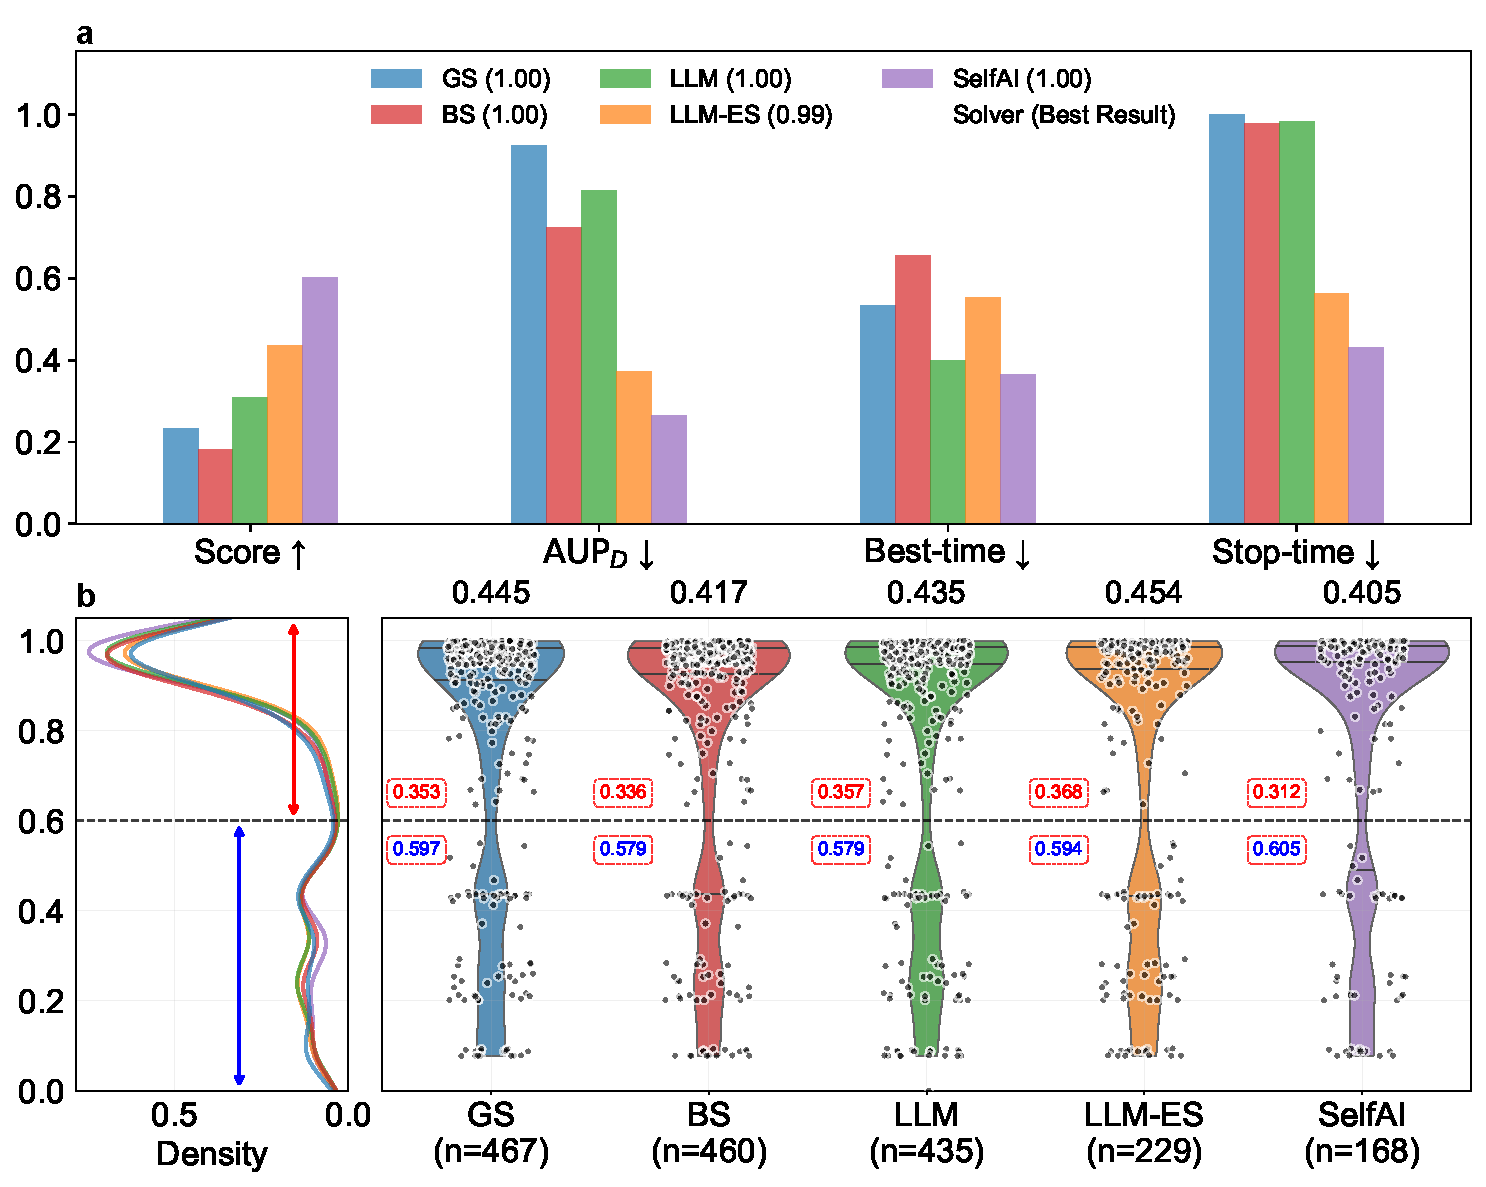
\includegraphics[width=0.7\linewidth]{figures/analysis/solver_performance_comparison2.pdf}
    \caption{\textbf{SelfAI Framework for Automated Scientific Experimentation.} \textbf{a}, Holistic architecture of the multi-agent system, which transforms various experiments in the research process into a structured workflow. \textbf{b}, User intents, comprising ideas and experiment schemes, are transformed into structured configurations via a predefined prompt. These inputs are processed through successive stages: hypothesis generation, strategic planning, trial execution, and result collection.}
    \label{fig:flowchart}
\end{figure*}